\documentclass[a4paper]{book}

%%% INICIO DEL PREÁMBULO %%%

\usepackage[utf8]{inputenc}
\usepackage[greek,spanish,es-tabla,es-nodecimaldot,es-noindentfirst]{babel}
\usepackage{babelbib}
\usepackage{nccmath}
\usepackage{amsthm}
\usepackage{lipsum}
\usepackage{tcolorbox}
\usepackage[thicklines]{cancel}
\usepackage{mathtools}
\usepackage{amssymb}
\usepackage{amsmath}
\usepackage{caption}
\usepackage{subcaption}
\usepackage{color}
\usepackage{verbatim}
\usepackage{enumerate}
\usepackage{geometry}
\geometry{a4paper,left=35mm,right=35mm,top=15mm,bottom=15mm}
\usepackage{isotope}
\usepackage{maybemath}
\usepackage{upgreek}
\usepackage{wasysym}
\usepackage[italic]{hepparticles}
\usepackage{subdepth}
\usepackage{siunitx}
\sisetup{
	mode 			= text,
	parse-units 	= false
}
\usepackage{physics}
\usepackage{braket}
\usepackage{tensor}
\usepackage{chemformula}
\usepackage{tikz}
\usepackage{url}
\usepackage{listings}
\usepackage{multirow}
\usepackage{multicol}
\usepackage[colorlinks=true]{hyperref}
\hypersetup{
	citecolor = blue,
	linkcolor = blue,
	urlcolor = blue,
	pdfauthor = {Javier Rodrigo López}
}
\usepackage{eso-pic}

% tikz
\usepackage{tikz} \usetikzlibrary{fit,babel,shapes,arrows,patterns,positioning,calc,decorations.pathmorphing,decorations.markings}
\tikzstyle{block} = [draw, fill=white, rectangle,
minimum height=3em, minimum width=6em]
\tikzstyle{sum} = [draw, fill=white, circle, node distance=1cm]
\tikzstyle{input} = [coordinate]
\tikzstyle{output} = [coordinate]
\tikzstyle{pinstyle} = [pin edge={to-,thin,black}]
\tikzset{
	block/.style = {draw, fill=white, rectangle, minimum height=3em, minimum width=3em},
	tmp/.style  = {coordinate},
	sum/.style= {draw, fill=white, circle, node distance=1cm},
	input/.style = {coordinate},
	output/.style= {coordinate},
	pinstyle/.style = {pin edge={to-,thin,black}}
}

\usepackage[oldvoltagedirection]{circuitikz}
\usepackage{pdflscape}

% Títulos
\usepackage{titlesec}
\titleformat{\section}{\normalfont\Large\bfseries}{\thesection}{1em}{}[{\titlerule[0.8pt]}]
% \renewcommand{\thesubsection}{\arabic{chapter}.\arabic{section}.\Alph{subsection}}
\titleformat{\subsubsection}{\normalfont\normalsize\bfseries}{\thesubsubsection}{1em}{}[{\titlerule[0.05pt]}]
\titlespacing{\section}{0pt}{2\parskip}{\parskip}
\titlespacing{\subsection}{0pt}{\parskip}{0pt}
\titlespacing{\subsubsection}{0pt}{\parskip}{0pt}

% Numeración de secciones
\setcounter{tocdepth}{2}
\setcounter{secnumdepth}{2}

% Figuras y descripciones
\renewcommand{\thefigure}{\arabic{figure}}
\renewcommand{\thesubfigure}{\Alph{subfigure}}
\captionsetup[figure]{labelfont={bf},name={Figura},labelsep=period}
\numberwithin{figure}{chapter}
\numberwithin{equation}{chapter}

% Enumerations
\newcounter{myenumi}
\renewcommand{\themyenumi}{\alph{myenumi})}
\newenvironment{myenumerate}{\setlength{\parindent}{0pt}\setcounter{myenumi}{0}\renewcommand{\item}{\par\refstepcounter{myenumi}\makebox[1.3em][l]{\themyenumi}}}{\par\bigskip\noindent\ignorespacesafterend}

% Own environments
\newenvironment{nota}{\underline{\textbf{NOTA:}} }{}
\newenvironment{caja}{\begin{tcolorbox}[colback = white, sharp corners, boxrule = 1 pt]}{\end{tcolorbox}}
\newtheorem*{conclusion}{Conclusión}
\newtheorem{teorema}{Teorema}
\newtheorem{definicion}{Definición}

% Para una bonita portada
\usepackage{wallpaper}
\usepackage{titling}
\usepackage{fancyhdr}
\pagestyle{fancy}
\setlength{\droptitle}{-10cm}
\renewcommand{\chaptermark}[1]{%
	\markboth{#1}{}}
\renewcommand{\sectionmark}[1]{%
	\markright{}}
\fancyhf{}
\fancyhead[LE,RO]{\bfseries\thepage} \fancyhead[LO]{\bfseries\rightmark} \fancyhead[RE]{\bfseries\leftmark} \renewcommand{\headrulewidth}{0pt} \renewcommand{\footrulewidth}{0pt} \addtolength{\headheight}{15pt}
\fancypagestyle{plain}{%
	\fancyhead{}
	\renewcommand{\headrulewidth}{0pt}
}

% Organización del texto
\newcommand{\formula}[1]{\vspace{13 pt}\noindent \textbf{\underline{#1}}}
\newcommand{\subtext}[1]{_{\text{#1}}}

% Unidades y utilidades varias
\renewcommand{\S}{\operatorname{S}}
\newcommand{\dB}{\operatorname{dB}}
\newcommand{\dBW}{\operatorname{dBW}}
\newcommand{\dBm}{\operatorname{dBm}}
\newcommand{\Hz}{\operatorname{Hz}}
\newcommand{\s}{\operatorname{s}}
\newcommand{\A}{\operatorname{A}}
\newcommand{\V}{\operatorname{V}}
\newcommand{\ohm}{\,\Omega}
\newcommand{\Pa}{\operatorname{Pa}}
\newcommand{\W}{\operatorname{W}}
\newcommand{\I}{\operatorname{I}}
\newcommand{\C}{\operatorname{C}}
\newcommand{\K}{\operatorname{K}}
\newcommand{\m}{\operatorname{m}}
\newcommand{\mm}{\operatorname{mm}}
\newcommand{\rad}{\operatorname{rad}}
\newcommand{\mol}{\operatorname{mol}}
\newcommand{\J}{\operatorname{J}}
\newcommand{\kg}{\operatorname{kg}}
\newcommand{\incremento}{\Delta}
\newcommand{\psus}{\, \ldots \,}
\newcommand{\mcm}{\operatorname{mcm}}
\newcommand{\MCD}{\operatorname{MCD}}
\renewcommand{\sin}{\sen}
\renewcommand{\arcsin}{\arcsen}
\renewcommand{\arctan}{\arctg}
\renewcommand{\min}{\operatorname{mín}}

\DeclarePairedDelimiter\evaluat{.}{\rvert}

% Vectores
\usepackage[c]{esvect}
\renewcommand{\vec}[1]{\vv{{#1}}}
\newcommand{\proy}[2]{\operatorname{proy}_{\vec{#2}}\vec{#1}}
\newcommand{\antiparallel}{\downharpoonleft \! \upharpoonright}
\newcommand{\parallelvec}{\upharpoonleft \! \upharpoonright}

% Espaciado
\usepackage{enumitem}
\setlist{before={\parskip=3pt}, after=\vspace{\baselineskip}}
\setlength{\parindent}{0pt}
\setlength{\parskip}{0.5em}

% Estadística
\DeclareMathOperator{\Var}{Var}
\DeclareMathOperator{\Cov}{Cov}
\renewcommand{\var}{\sigma ^2}
\DeclareMathOperator{\B}{B}
\DeclareMathOperator{\BN}{BN}
\DeclareMathOperator{\Geo}{Geo}
\DeclareMathOperator{\Poisson}{Poisson}
\DeclareMathOperator{\U}{U}
\DeclareMathOperator{\Exp}{Exp}
\DeclareMathOperator{\N}{N}
\DeclareMathOperator{\Mult}{Mult}
\newcommand{\TF}[1]{\mathrm{TF} \left\lbrace \left. #1 \right\rbrace \right.}
\newcommand{\probCond}[2]{P \left( #1 \: \middle\vert\:  #2 \right) }

% Electromagnetismo y Ondas
\newcommand{\errorGrave}{\textbf{FG!!!}}
\newcommand{\mas}{M.A.S.}
\newcommand{\mcu}{M.C.U.}
\newcommand{\ed}{E.D.}
\newcommand{\edmas}{E.D. del M.A.S.}
\usepackage{esint}

% Señales y Sistemas
\renewcommand{\H}{H}

% Circled number
\newcommand{\circledNumber}[1]{\raisebox{.9pt}{\textcircled{\raisebox{-.9pt}{#1}}}}

% Footnotes
% \renewcommand{\thefootnote}{\fnsymbol{footnote}}

% Ejemplo
\newcounter{elejemplo}
\newcommand{\ejemplo}[2]{
	\refstepcounter{elejemplo}
	\begin{center}
		\fbox{\begin{minipage}{0.85\linewidth}
			\textbf{Ejemplo \arabic{elejemplo}.} #1
			\begin{center}
				\underline{\textbf{Solución}}
			\end{center}
			#2
		\end{minipage}}
	\end{center}
}

% Repeticiones
\usepackage{forloop}
\newcommand{\repvec}[3]{
	\foreach \uwu in {1,...,#2}
		{\vec{#1}_{\uwu} ,}
	\, \ldots \, , \vec{#1}_{#3}
}
\newcommand{\rep}[3]{
	\foreach \uwu in {1,...,#2}
		{#1_{\uwu} ,}
	\, \ldots \, , #1_{#3}
}
\newcommand{\repinf}[3]{
	\foreach \uwu in {#2,...,#3}
		{#1_{\uwu} ,}
	\, \ldots
}

%%% FIN DEL PREÁMBULO %%% % Se incluye el preámbulo

% Título y portada
\title{\Huge Fundamentos de Sonido e Imagen\\\vspace*{5pt}
\Large Apuntes de clase}
\author{Javier Rodrigo López \thanks{Correo electrónico: \href{mailto:javiolonchelo@gmail.com}{\texttt{javiolonchelo@gmail.com}}}} 
\date{\today}

%%% INICIO DEL DOCUMENTO %%%
\begin{document}

\setlength{\wpYoffset}{1cm}
\ThisCenterWallPaper{0.7}{./Imágenes/Sorolla.jpg}
\maketitle

% Marca de agua
\AddToShipoutPictureFG{
\begin{tikzpicture}[overlay,remember picture]
\path (current page.south west) -- (current page.north east)
 node[midway,scale=8,color=lightgray,sloped,opacity=0.05] {Javier Rodrigo López};
\end{tikzpicture}
}

% Logotipos UPM y ETSIST
\begin{figure}[t!]
\centering
	\begin{subfigure}[b]{0.65\linewidth}
		
\includegraphics[width=\linewidth]{../../Archivos comunes/upm_logo.png}
	\end{subfigure}
	\begin{subfigure}[b]{0.25\linewidth}
		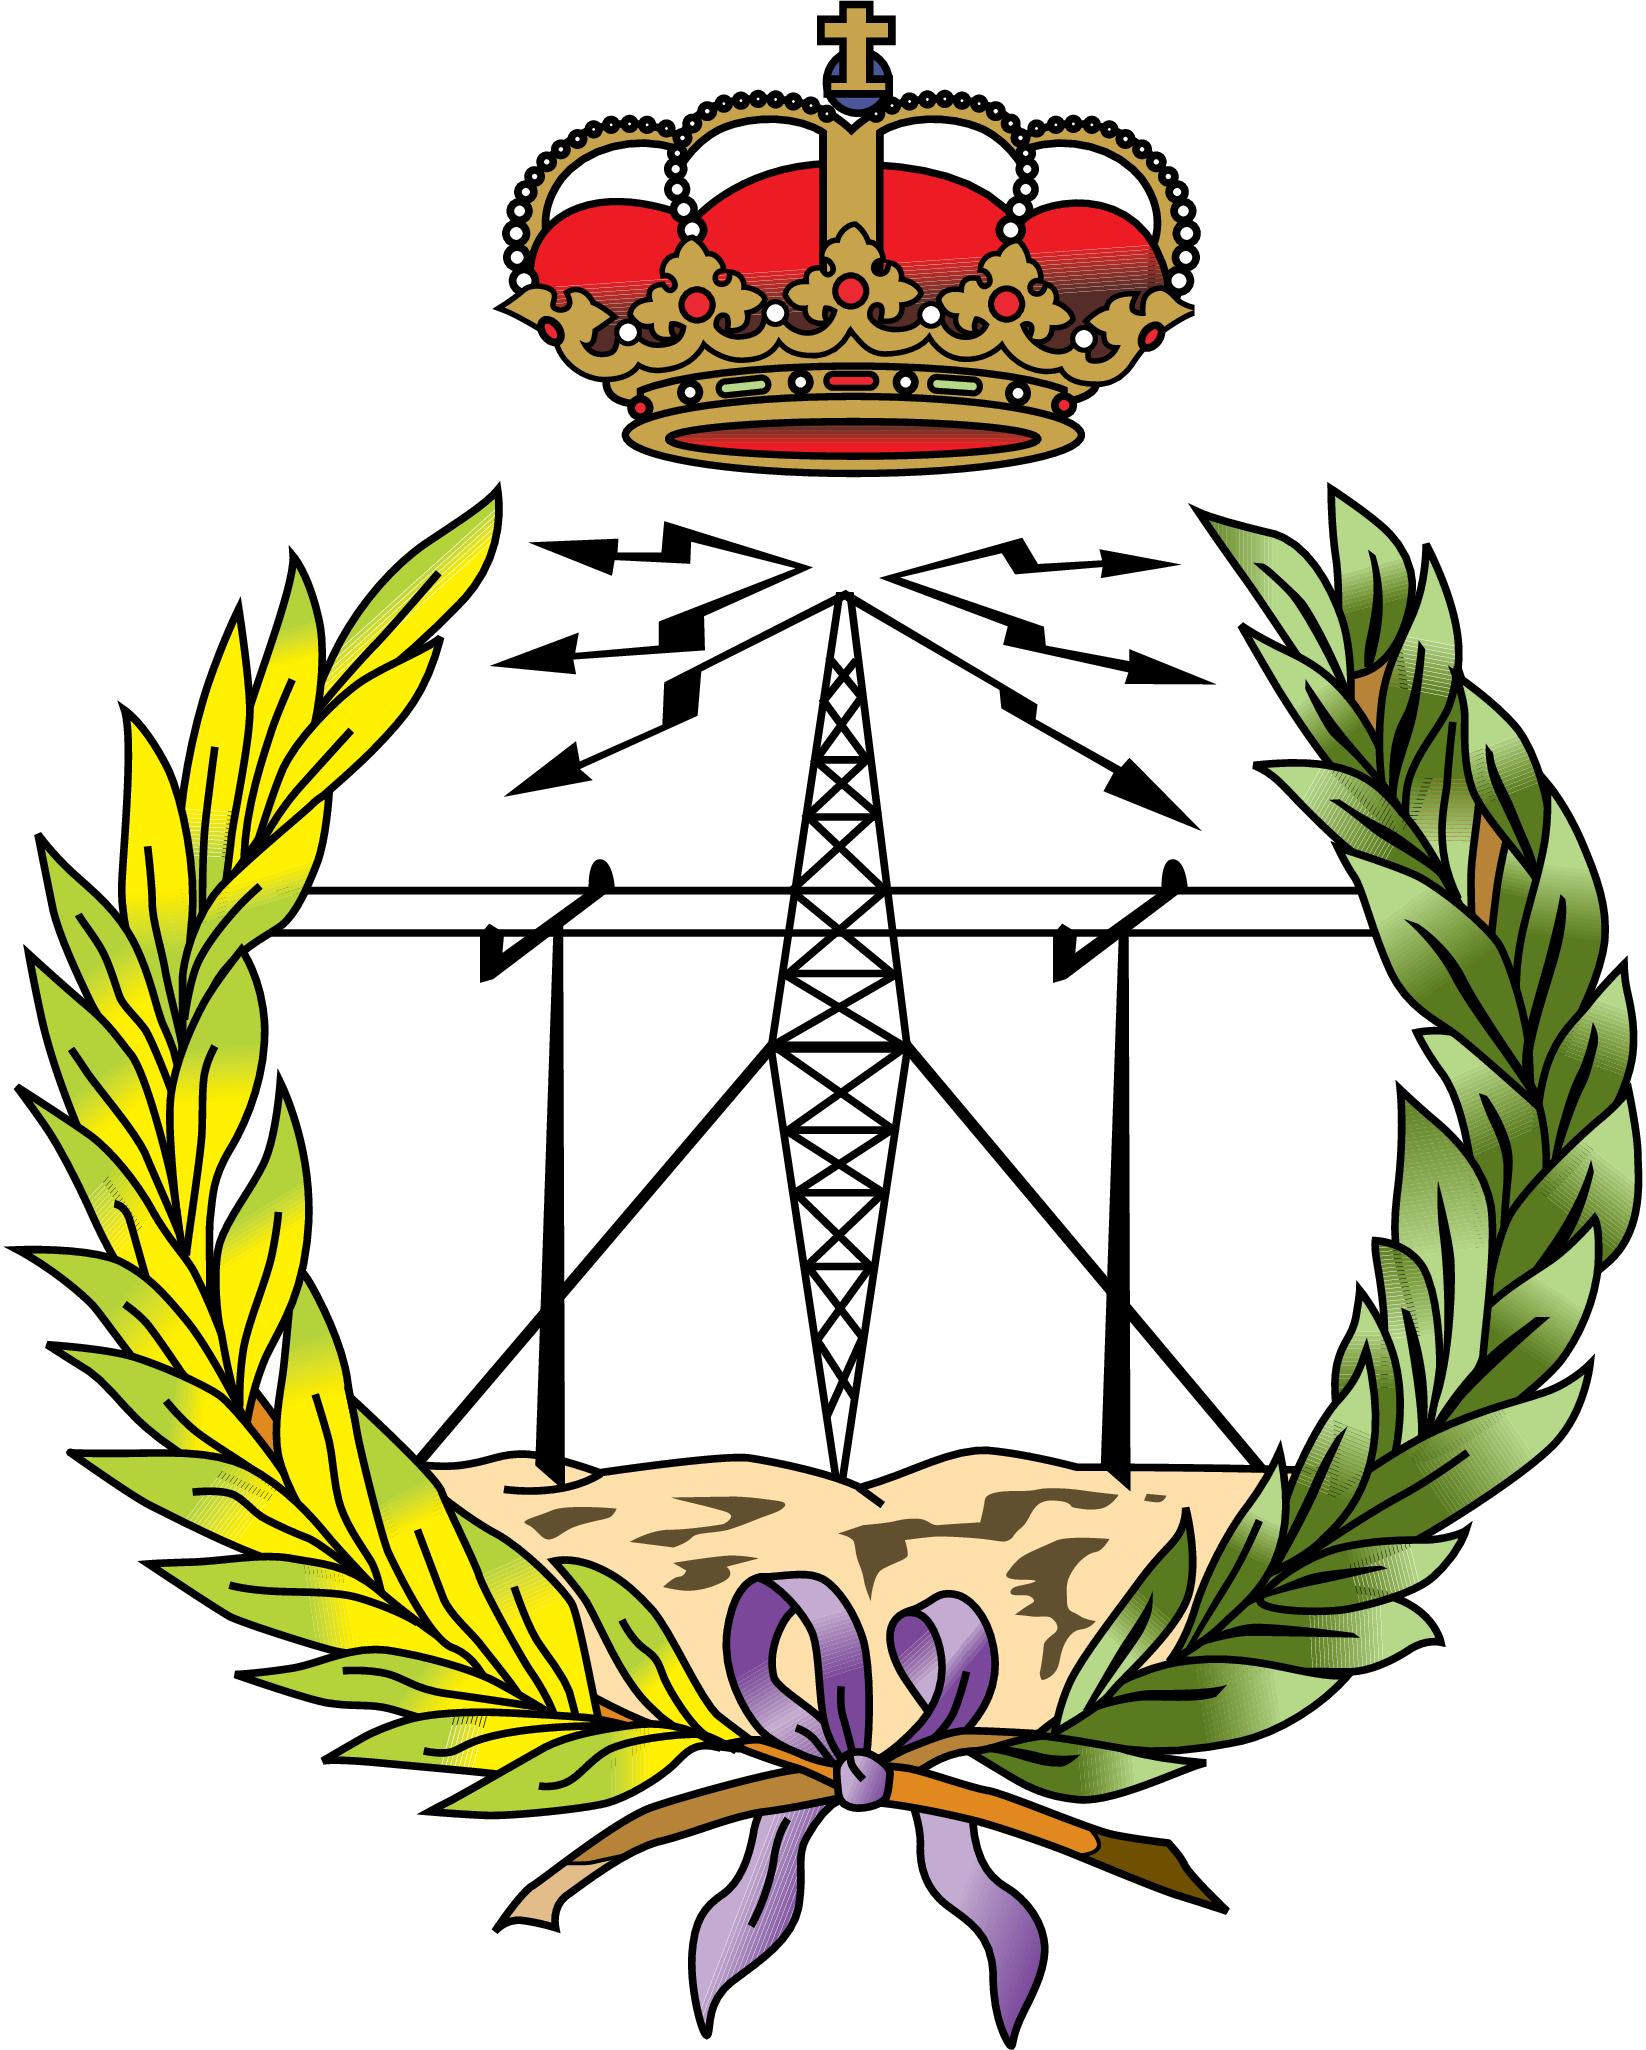
\includegraphics[width=\linewidth]{../../Archivos comunes/etsist_logo.png}
	\end{subfigure}
\end{figure}

% Introducción
\newpage
\phantomsection
\addcontentsline{toc}{section}{Introducción}
\section*{Introducción}
Imagen de la portada: \textsl{Corriendo por la playa. Valencia}, de Joaquín Sorolla.

Información para los sentidos de la vista y el oído:
\begin{itemize}
	 \item Luz $\longrightarrow$ Imagen $\longrightarrow$ Vídeo
	 \item Vibraciones $\longrightarrow$ Sonido $\longrightarrow$ Audio
\end{itemize}

\begin{itemize}
	 \item \textbf{Consumo audiovisual}: Consumo humano
	 \item \textbf{Análisis}: Procesado, Edición, Interpretación.
	 \item \textbf{Síntesis}: Generación, automatización
\end{itemize}

Luz, óptica, fotometría  Magnitudes físicas: Propagación, fuentes, medio, obstáculos
Ondas, vibraciones, sonido, acústica 
S.V. Humano. Color PERCEPCIÓN HUMANA y COMPRENSIÓN Psicoacústica
Cámaras, scanners, pantallas, impresión, scanners médicos

\textbf{Usuario}: Utiliza equipo o servicio. Creador de contenido. Artista.
\textbf{Técnico}: Operar, mantener instalaciones
\textbf{Ingeniero}:
\begin{itemize}
	 \item Conocimientos básicos fuertes
	 \item Capacidad de trabajo
	 \item Adaptabilidad e Independencia
	 \item Comunicación: Oral, Escrita y en inglés
	 \item Cooperación: Trabajo con otros
	 \item Aprendizaje continuo, curiosidad
	 \item Investigación: Crear algo nuevo
	 \item Experiencia: Intuición, "sabiduría"
\end{itemize}

Imagen: 

Teoría: 16h + 2h parcial
Laboratorio: 8h = 4 prácticas online

Sonido:

Teoría 18h online
Laboratorio (Aula L8103) 4h = 2 prácticas presenciales

\subsubsection{Evaluación}
Teoría Imagen: 35\% + Teoría Sonido 35\% + cada laboratorio cuenta 15\%

Hay que sacar más de un 5 en cada parte.

\newpage

% Índice (TOC)
\setlength{\parskip}{0em}
\tableofcontents 
\setlength{\parskip}{0.5em}

%%% INICIO DE LOS APUNTES %%%
\chapter{Señales, sistemas y medidas acústicas. Revisión de conceptos}

\chapter{Señales acústicas}
\section{Valor RMS y nivel de una señal}
\section{Serie de Fourier y Transformada de Fourier}
\section{Densidad espectral de potencia}
\section{Nivel espectral y nivel en banda}
\section{Ruido blanco y ruido rosa}
\section{Sistemas y medidas acústicas}
\section{Sistema lineal. Función de transferencia. Respuesta al impulso}
\section{Métodos de análisis de sistemas}
\section{Analogías electro-mecánico-acústicas}

\chapter{Audición y voz}
\section{Fisiología y funcionamiento del sistema auditivo humano}
\section{Características de la respuesta auditiva}
\section{No linealidad del sistema auditivo}
\section{Efecto de enmascaramiento temporal y frecuencial}
\section{Audición binaural}
\section{Mecanismo de generación de la voz}
\section{Características acústicas de voz}
\section{Análisis de la señal de voz}

\chapter{Ondas planas y esféricas}
\section{Ecuación de onda plana. Velocidad de propagación}
\section{Velocidad vibratoria e impedancia de una onda plana}
\section{Presión e intensidad acústicas}
\section{Ecuación de una onda esférica}
\section[Velocidad vibratoria e impedancia de una onda esférica]{Velocidad vibratoria e impedancia de una onda\\ esférica}
\section{Campo acústico originado por una fuente. Divergencia esférica}
\section{Potencia radiada por una fuente}

\chapter{Ondas estacionarias}
\section{Reflexión de una onda plana}
\section{Impedancia de una línea de transmisión acústica}
\section{Intensidad acústica de una onda estacionaria}
\section{Transmisión acústica a través de varios medios}

\chapter{Formación y captación de imágenes}

\section{Introducción}

\subsection{Diferencias y similitudes entre las vista y el oído}
\begin{itemize}
	 \item Ambas tienen alcance cercano y lejano.
	 \item El detalle espacial es alto en la vista y bajo en el oído.
	 \item Ambos tienen alto detalle temporal.
	 \item La vista tiene un bajo detalle frecuencial (colores) mientras que el oído tiene un alto detalle frecuencial (tono y timbre).
	 \item Ambas sensaciones comienzan y acaban rápidamente.
\end{itemize}

Llamamos \textbf{luz} a la parte del espectro electromagnético visible por el Sistema Visual Humano. Comprende aproximadamente las longitudes de onda entre 380nm y 780nm.

Llamamos \textbf{sonido} al rango de frecuencias de las vibraciones audibles por el Sistema Auditivo Humano. Comprende frecuencias entre 20Hz y 20kHz.

La propagación de ambos es en forma de ondas, por lo que se puede relacionar la frecuencia, la velocidad de propagación y la longitud de onda:
\[ \lambda = \frac{v}{f}  \]

La velocidad de propagación de la luz es aproximadamente un millón de veces mayor que la del sonido. Sin embargo, el rango de frecuencias de sonido es mucho mayor que el de la luz.

La interacción con medio y obstáculos depende de los rangos de longitud de onda.

Estudiaremos:
\begin{itemize}
	 \item Física en general.
	 \item Óptica geométrica.
	 \item Fotografía: Captura de imágenes.
	 \item Fotometría: Medida de energía transportada, fuentes y objetos iluminados.
	 \item Visión humana y colorimetría.
\end{itemize}

\section{Óptica geométrica}

Trata sobre reflexión y refracción de luz en fronteras entre medios y su propagación en medios homogéneos.

Simplificación

Medio homogéneo: mismas propiedades en todos los puntos. Viaja en línea recta.

Sucesión de medios homogéneos: Lentes.

Campo luminoso. En un momento dado en un punto del espacio hay:
\begin{itemize}
	 \item Rayos en todas direcciones, provenientes de:
	 \begin{itemize}
		  \item Fuentes de luz
		  \item Superficies
		  \item Atmósfera
	 \end{itemize}
\end{itemize}

Cámara oscura y modelo de cámara ideal. Es una caja o habitación con apertura muy pequeña. Desde cada punto a la vista solo pasa luz en una dirección y genera una imagen nítida e invertida en el interior. "Rayo único".

Es el modelo de cámara ideal usado en Gráficos 3D.



\subsubsection{Cámara estenopeica. \textit{Pinhole}.}

El eje $Z$ es perpendicular al eje óptico o eje de la cámara. FALTA AÑADIR IMAGEN

Sensor: tamaño y relación de aspecto.

El tamaño se mide en milímetros.

La relación de aspecto es el ancho entre el alto. Si el objeto es muy grande o está muy cerca, su imagen puede no caber en el sensor.

Círculo de confusión:

En realidad, de cada punto de la vista se proyecta un cono de rayos con la forma de la apertura: círculo de confusión.

Para que la imagen sea nítida basta con que el círculo de confusión sea menor que el tamaño de un fotodetector del sensor.

Por ello, para este modelo de cámara se supone que pasa un único rayo por la apertura.

\subsubsection{Ejercicios}

Para resolver los ejercicios con cámaras estenopeicas, utilizaremos el \textbf{teorema de Tales}. Siendo estas las distancias

EJERCICIO 1
Se cuenta con una cámara que se ajusta el modelo de cámara estenopeica ideal. El tamaño de su sensor de imagen es 36x24 mm 

\subsubsection{Sensor de Imagen} 

Capta energía luminosa mediante:
\begin{itemize}
	 \item Proceso fotoquímico. Se debe a una reacción química.
	 \item Proceso fotoeléctrico. Cada celda (pixel) del sensor se carga eléctricamente de forma proporcional a la energía luminosa recibida.
\end{itemize}

A más energía luminosa, más brillo en la imagen capturada.

\subsubsection{Deventajas de la cámara estenopeica}

Al entrar muy poca luz, la energía luminosa que recibe el sensor de la cámara estenopeica

Aspectos clave al capturar una imagen
\begin{itemize}
	 \item Imagen enfocada (nítida) para aperturas mayores. Necesitamos óptica de enfoque.
	 \item Cantidad de luz suficiente, depende de:
	 \begin{itemize}
		  \item Luz presente en la escena
		  \item Tamaño de la apertura
		  \item Tiempo de exposición (relacionado con la velocidad de obturación o \textit{shutter})
	 \end{itemize}
\end{itemize}

Velocidad de la luz e índice de refracción.

La propagación de la luz en un 

Refracción en superficie esférica.

La potencia focal.

Ecuación de lente delgada
\[ P=\frac{1}{d_f}=\left( n_l-n_o \right) \cdot \left( \frac{1}{R_1} - \frac{1}{R_2}  \right)  \]

Convención de signos y geomtría.

\section{Fotografía}

\section{Fotometría}

\chapter{El sistema visual humano. Colorimetría}
\section{Introducción a la visión}
\section{Estructura y óptica del ojo humano}
\section{La retina, nuestro sensor}
\section{Percepción: Implicaciones en los sistemas de imagen}

\chapter{Señales utilizadas para la representación de imágenes}
\section{Modelos cromáticos para el almacenamiento cuantificado de los colores}
\section{Señales de luminancia y de crominancia}
\section{Importancia concedida por el ojo a las señales de luminancia y crominancia}
\section{Cartas de barras para los estudios cromáticos de imágenes fijas y de vídeo}
\section{Relación de aspecto y exploraciones progresivas y entrelazada}
\section[Resolución horizontal y vertical de las imágenes (SD, HD, UHD)]{Resolución horizontal y vertical de las imágenes\\ (SD, HD, UHD)}
\section{Señales normalmente utilizadas para la transmisión de señales de vídeo}
\section{Intervalos de vídeo e intervalos de sincronismo}

\appendix

\chapter{Prácticas}
\section[Introducción. Técnicas de medidas acústicas. Técnicas de análisis de sistemas mecánicos y acústicos]{Introducción. Técnicas de medidas acústicas.\\ Técnicas de análisis de sistemas mecánicos y acústicos}
\section{Osciladores mecánicos y acústicos}
\section{Ondas acústicas esféricas. Potencia radiada por una fuente}
\section{Ondas acústicas estacionarias. Impedancia acústica. Impedancia de radiación de un tubo}
\section{Imagen digital}
\section{Relación de aspecto y adaptaciones}
\section{Brillo y contraste}
\section{Color. Saturación y tinte}
%%% FIN DE LOS APUNTES %%%

%%% BIBLIOGRAFÍA %%%
% Por defecto, se encuentra desactivada. Esto disminuye el tiempo de procesado. Se puede activar cuando se vaya a exportar el PDF definitivo

%\newpage
%\phantomsection
%\label{sec:bibliografia_final}
%\renewcommand{\refname}{Bibliografía}
%\addcontentsline{toc}{section}{Bibliografía}
%\bibliography{bibliografia} % Nombre del archivo (sin ".bib")
%\bibliographystyle{bababbrv} 
\end{document}
